\chapter{One-way Analysis of Variance}
We know how to test fit the difference in 2 means
\begin{align*}
    H_0 &: \mu_1 = \mu_2 \qquad \text{i.e} \qquad \mu_1 - \mu_2 = 0.\\
    H_a &: \mu_1 \neq \mu_2  \qquad \text{i.e} \qquad \mu_1 - \mu_2 \neq 0
\end{align*}
Now we endeavor to construct a test to detect difference in means over multiple groups.

\example* 24 expert typists test three new keyboard designs. Randomly assign 8 to each type of keyboard and assigned the same document to type up. The time of the task is recorded with the idea that a group with significantly less time on task would imply a better keyboard design
  \begin{center}
    \begin{tabular}{|c|c|}
         \hline
         design & times\\
         \hline
         KB1 & 364 366 394 386 379 398 371 370\\
         KB2 & 355 359 374 342 378 355 376 358\\
         KB3 & 360 345 374 390 386 373 393 366\\
         \hline
    \end{tabular}
\end{center}
An obvious stat to look at is means
$$\bar{A} = 378.5 \qquad \bar{B} = 362.125 \qquad \bar{C} = 373.375$$
$B$ \say{looks} better, but can we design a test to determine if it is \say{significantly} so? This is our goal.

\nl The standard null hypothesis is that the true population means are the same for each group, $H_0: \mu_1 = \mu_2 = \cdots = \mu_k = \mu_0$. The alternative $H_a$ is that at least one of the $\mu_i$'s are different.

\nl Notation: Let $i$ indicate the \say{group}. E.g. $k_i$ with $i = 1, 2, 3$. ($k$ for keyboard). Let $j$ denote the data point in that group. i.e. $Y_{1\,3} = 394$, $Y_{2\,5} = 378$.

\nl Let $n_i$ be the number of data points in the $i^{\text{th}}$ group. Here $n_1 = n_2 = n_3 = 8$. Let $n$ be the total of all data points. $n = \sum_{i=1}^k n_i$. Here $n = 24$.

\nl Formally, we assume $Y_{i\,j} \sim N(\mu_i, \sigma^2)$ where each group has mean $\mu_i$, but all groups have the same variance $\sigma^2$.
\\We need a stat.

\nl To find \say{a} stat, we construct a likelihood ratio test. For $H_0$ we have our usual MLEs. If there is only $\mu_0$
$$\muh_0 = \over{n} \sum_{i=1}^k \sum_{j=1}^{n_i} Y_{i\,j}$$
and $${S_0}^2 = \sum_{i=1}^k \sum_{j=1}^{n_i} (Y_{i\,j} - \muh_0)^2.$$
Under the alternative hypothesis, for the individual means, we again use the standard MLE
$$\muh_i = \over{n_i}\sum_{j=1}^{n_i} Y_{i\,j} = \bar{Y_i}.$$
Aside: In our motivational example, $\bar{A} = \bar{Y_1} = 378.5$, $\bar{B} = \bar{Y_2} = 362.125$, etc.

\nl But we are still assuming a unique $\sigma^2$ for all groups. So the MLE for $$S_a^2 = \over{n} \sum_{i=1}^k \sum_{j=1}^{n_i} (Y_{i\,j} - \muh_i)^2.$$
Remark: Proving that this is an MLE is a good review and will be coming to a homework soon.

\nl Construct a likelihood function:
\begin{align*}
    L(\text{All } Y_{i\,j} \mid \muh_0, S_0^2) &= \prod_{i=1}^k \prod_{j=1}^{n_i} \pover{2\pi S_0^2}^{1/2} \exp \pfrac{-(Y_{i\,j - \muh_0})^2}{2S_0^2}\\
    &= \pover{2\pi S_0^2}^{n/2} \exp \pars{- \over{2S_0^2} \sum_{i=1}^k \underbrace{\sum_{j=1}^{n_i} (Y_{i\,j} - \muh_0)^2}_{\textstyle nS_0^2}}\\
    &= \pover{2\pi S_0^2}^{n/2} \exp \pars{- \frac{nS_0^2}{2S_0^2}}\\
    &= \pover{2\pi S_0^2}^{n/2} e^{-n/2}
\end{align*}
Under $H_a$, same \say{algebra} occurs.
$$L(\text{All } Y_{i\,j} \mid \muh_0, S_a^2) =  \pover{2\pi S_a^2}^{n/2} e^{-n/2}$$
Then the ratio of likelihood functions yields
$$\frac{
    L(\text{All } Y_{i\,j} \mid H_0)
}{
    L(\text{All } Y_{i\,j} \mid H_a)
} = \frac{
    \pover{2\pi S_0^2}^{n/2} e^{-n/2}
}{
    \pover{2\pi S_a^2}^{n/2} e^{-n/2}
} = \pfrac{S_a^2}{S_0^2}^{n/2} < k$$
Implies the statistic $T = \dfrac{S_a^2}{S_0^2}$ and small values of $T$ support the alternative hypothesis (define our RR). This makes sense because if the true means are different then $S_a^2$ will be the correct estimator for $\sigma^2$ and $S_0^2$ will be larger (on average).

\nl We have a problem\dots This is an entirely new stat for us.

\nl One thing we should show is that (a)
$$S_a^2 \text{ is an estimator of } \sigma^2$$
moreover, we need it unbiased.

\nl Note that via multiplying by the correct degrees of freedom $\nu$, and dividing by $\sigma^2$, the numerator and denominator are $\chi^2$ distributed. This lead to the advent of the $F$-distribution.

\nnl Topic: The $F$-distribution. Suppose $X_1 \sim \chi^2(m)$ and $X_2 \sim X^2(n)$ and are independent. Define
$$Y_i := \frac{X_1\big/  m}{X_2 \big/ n}$$
to be an $F$ random variable with $m$ numerator degrees of freedom and $n$ denominator degrees of freedom. We usually write $Y_i \sim F(m,n)$.

\nl The derivation is akin to the derivation of the $T$-stat. We used the Jacobian method of transformations. ($\S6.6$ in the text. This is usually skipped in MTH 325.)

\nl Letting $Y_2 = X_2$, we can find the joint density function of $Y_1$ and $Y_2$, then we integrate the joint density to get the marginal density of $Y_i$\dots
$$
    f(y_1) = \dfrac{
        \Gamma \pfrac*{m+n}{n}
    }{
        \Gamma \pfrac*{m}{2} \Gamma \pfrac*{n}{2}
    } \pfrac{m}{n}^{n/2}
    \frac{
        y_1^{m/2 -1}
    }
    {
        \pars{1 + \pfrac*{my_1}{n}^{(m+n)/2}}
    } \text{ and } y_i > 0.
$$

%"last day" picture
\nl \textbf{Last day:} Looking at at designing a test $H_0 : \mu_1 = \mu_2 = \cdots = \mu_k = \mu_0$ versus $H_a$ not all equal.

\nl Theorem: Likelihood ration, find a new (for us) statistic that looked like a $\dfrac{\chi^2 \text{ r.v.}}{\chi^2 \text{ r.v.}}$. This lead us to the $F$-distribution.

$$Y \sim F(m,n) \qquad \text{when} \qquad Y = \frac{X_1/m}{X_2/n}$$
and
$$X_1 \sim \chi^2(m) \wideand X_2 \sim \chi^2(n).$$
Graph $f(y), y >0$:
\notab{
    \begin{center}
        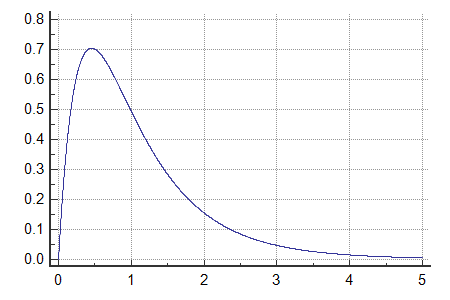
\includegraphics[width=3in]{F_graph.png}
    \end{center}
}

\nl For $\E{Y}$ and $\Var{Y}$.
\begin{align*}
    \E{Y} &= \E{ \frac{X_1/m}{X_2/n}}\\
    &= \E{\frac{n}{m}\cdot \frac{X_1}{X_2}}\\
    &= \frac{n}{m} \E{X_1 \cdot \over{X_2}}\\
    &= \frac{n}{m} \E{X_1} \E{\over{X_2}} \tag{by independence}\\
    &= \frac{n}{m} \cdot m \E{\over{X_2}}\\
    &= n \E{\over{X_2}} \tag{numerator df has no impact}\\
    &= n \cdot \underbrace{\over{n-2}}_{\text{by thm.}}
\end{align*}
$$\E{Y} = \frac{n}{n-2}.$$
Also, with proof omitted,
$$\Var{Y} = \frac{2n^2 (m+n-2)}{n(n-2)^2(n-4)}.$$
End $F$-distribution background. Then,
$$T = \frac{{S_0}^2}{{S_a}^2} = \frac{
    \over{n} \sum_{i=1}^k \sum_{j=1}^{n_i} (Y_{i\,j} - \muh_0)^2
}{  \over{n} \sum_{i=1}^k \sum_{j=1}^{n_i} (Y_{i\,j} - \muh_i)^2}$$
and the $\over{n}$ can cancel. If $S_0^2$ and $S_a^2$ were independent, then dividing by their degrees of freedom would yield an $F$-distribution. Sadly, they aren't. But we can algebra to independent ratios. Start with the top,
\begin{align*}
    {S_0}^2 &=  \sum_{i=1}^k\sum_{j=1}^{n_i} (Y_{i\,j} - \muh_0)^2\\
    &= \sum_{i=1}^k \sum_{j=1}^{n_i} \pars{(Y_{i\,j} - \muh_i) + (\muh_i - \muh_0)}^2\\
    &= \sum_{i=1}^k \sum_{j=1}^{n_i} \brac {
        (Y_{i\,j} - \muh_i)^2 + 2(Y_{i\,j- \muh_i})(\muh_i - \muh_0) + (\muh_i - \muh_0)^2
    }\\
    &=  \sum_{i=1}^k \sum_{j=1}^{n_i} (Y_{i\,j} - \muh_i)^2 + 2 \sum_{i=1}^k \bigbrac{
        (\muh_i - \muh_0) \underbrace{
            (Y_{i\,j} - \muh_i)
        }_{
            \substack{= 0\text{ as it's the} \\ \text{sum of all} \\ \text{deviations for} \\ \text{mean within a} \\ \text{group from group mean}}
        }
    } + \sum_{i=1}^k n_i( \muh_i - \muh_0 )^2\\
    &= \sum_{i=1}^k \sum_{j=1}^{n_i} (Y_{i\,j} - \muh_i)^2 + \sum_{i=1}^k n_i( \muh_i - \muh_0 )^2\\
    &= {S_a}^2 +  \sum_{i=1}^k n_i( \muh_i - \muh_0 )^2
\end{align*}
Then
$$\frac{{S_0}^2}{{S_a}^2} = 1 + \frac{
    \sum_{i=1}^k n_i (\muh_i - \muh_0)^2
}{
    \sum_{i=1}^k \sum_{j=1}^{n_i} (Y_{i\,j} - \muh_i)^2
}$$
We are pretty close to independence. Recall we have Fisher's Theorem:
 $\chi^2 \sim N(\mu, \sigma^2)$ then $\Xbar$ and $S^2$ are independent random variables and $\Xbar \sim N(\mu, \sigma^2/n).$
 $$(n-1)\frac{S^2}{\sigma^2} \sim \chi(1)$$
Thus the $\muh_i$'s up top are independent of all the variances ${S_i}^2$ in sum of the denominator. Also, $\muh_0$ \underline{is} a function of $\muh_i$
$$\muh_0 = \frac{
    n_1 \muh_1 + n_2 \muh_2 + \cdots + n_k \muh_k
}{n}$$
And the entire numerator is independent of the variance terms in the numerator when $H_0$ is true. Now, when $H_0$ is true, all the resultant variable (top and bottom) are $\chi^2$ distributed. The last thing to do is figure out degrees of freedom. Given $\mu_0$,
$$\frac{\muh_1 - \mu_0}{\sigma / \sqrt{n_i}} \sim N(0,1) \wideand \frac{n_i(\muh_i - \mu_0)^2}{\sigma^2} \sim \chi^2(1)$$
So, the sum of $\chi^2$ random variables is also a $\chi^2$ rv and the degrees of freedom add. Thus
$$\over{\sigma^2} \sum_{i=1}^k n_i (\muh_i - \mu_0)^2 \sim \chi^2(k).$$
On the other hand, to use these facts, use the say \say{trick} again
$$\muh_1 - \mu_0 = \red{(} \muh_1 - \muh_0 \red{)} + \red{(} \muh_0 - \mu_0 \red{)}$$
And
$$\sum_{i=1}^k n_i (\muh_i - \mu_0)^2 = \underbrace{
\sum_{i=1}^k n_i (\muh_i - \muh_0)^2
}_{
    \text{the numerator}
} + n \underbrace{
    (\muh_0 - \mu_0)^2
}_{
    \substack{\text{divide by } \sigma^2, \\ \text{this is } \chi^2(1)}
}$$
In the end
$$\underbrace{
    \over{\sigma^2} \sum_{i=1}^k n_i (\muh_i - \mu_0)^2
}_{\textstyle \chi^2(k)} = \underbrace{
    \over{\sigma^2}  \sum_{i=1}^k n_i (\muh_i - \muh_0)^2
}_{
    \substack{\text{the numerator is} \\ \textstyle \chi^2(k-1)}
} + \underbrace{
    n\frac{ (\muh_0 - \mu_0)^2}{\sigma^2}
}_{\textstyle \chi^2(1)}$$
Denominator is much easier,
$$\sum_{i=1}^k \underbrace{\sum_{j=1}^{n_i} \frac{(Y_{i\,j} - \mu_i)^2}{\sigma^2}}_{\textstyle {S_i}^2 \sim \chi^2(n_i - 1)}$$
and by independences, summing all the $\chi^2(n_i -1)$ variables yield a
$$\chi^2 \underbrace{\pars{\sum_{i=1}^k (n_i - 1)}}_{\text{add all \df}} = \chi^2(n-k)$$
This is a ton of work, but in the end we have
$$F = \frac{
    \sum_{i=1}^k n_i (\muh_i - \mu_0)^2 \Big/ k-1
} {
    \sum_{i=1}^k \sum_{j=1}^{n_i} (Y_{i\,j} - \muh_i)^2 \Big/ n-k
} \sim F(k-1,\, n-k)$$
when $H_0$ is true.

\nl Topic: The ANOVA test.
\begin{enumerate}[label=\textcircled{\raisebox{-1pt}{\arabic*}}]
    \item Compute the null and alternative estimate of all the sample means.
    \item Use these to compute the sum of squares in our $F$-statistic
    \item Construct a table (R or Excel?) to compute the $p$-value.\\$F_{\text{obs}}$ is $F$ observed. We computed this.
    $$\P{F > F_{\text{obs}}},\; F - F(k-1,n-k)$$
    \notab{
    \begin{center}
        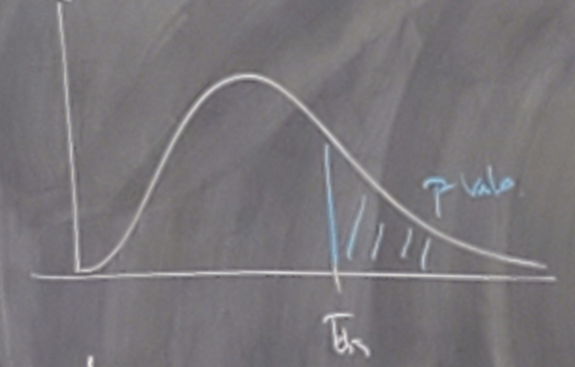
\includegraphics[width=3in]{upperTail_F.png}
    \end{center}
}
    \item Conclusion. There is standard language for all this. In the denominator,
    $$\SSW = \sum_{i=1}^k \sum_{j=1}^{n_i} (Y_{i\,j} - \muh_i)^2$$
    the sum of squares \underline{WITHIN} a group. And the numerator
    $$\SSA = \sum_{i=1}^k n_i (\muh_i - \mu_0)^2$$
    the sum of the squares \underline{AMONG} groups. A measure of variance among the sample means. Recall originally,
    $$\frac{{S_0}^2}{{S_a}^2} = \frac{{S_a}^2 + \SSA}{\SSW}$$
    Thus we showed the factorization yield \underline{total variation}.
    $$S_{0}^2 = \SSW + \SSA \qquad \text{or} \qquad \SST = \SSW + \SSA$$
\end{enumerate}

%F observed = Fobs start of 4/22
\nnl ANOVA Test
$$\SSA = \sum_{i=1}^k n_i (\muh_1 - \muh_0)^2 \qquad \text{(SS among groups)}$$
$$\SSW = \sum_{i=1}^k \sum_{j=1}^{n_i} (Y_{i\,j} - \muh_i)^2 \qquad \text{SS within groups}$$
$${S_0}^2 = \SST = \SSA + \SSW$$
$$R^2 = \frac{\SSA}{\SST} \quad \text{coef. of determination}$$

\nl Discussion: The ANOVA table
% Source | SS  |  df | MS      | F_obs   | p value
% -------+-----+-----+---------+---------+
% among  | SSA | k-1 SSA/(k-1) | MSA/MSW | P(F(k-1,n-k)>F_obs)
% within | SSW | n-k SSW/(n-k) |
% total  | SST | n-1

  \begin{center}
    \begin{tabular}{|l|c c c c c|}
         \hline
         Source & SS & df & Mean Squares & $F_{\text{obs}}$ & $p$-value\\
         \hline
         among & $\SSA$ & $k-1$ & $\SSA/(k-1)$ & $\operatorname{MSA}/\operatorname{MSW}$ & $\P{F(k-1, n-k) > F_{\text{obs}}}$ \\
         within & $\SSW$ & $n-k$ & $\SSW/(n-k)$ & & \\
         total & $\SST$ & $n-1$ & & &\\
         \hline
    \end{tabular}
\end{center}

\example*
\begin{center}
    \begin{tabular}{|l|c c c|}
         \hline
         Treatment & & Data & \\
         \hline
         1 & 2 & 4 & 3 \\ 2 & 6 & 4 & \\ 3 & 3 & 5 & 4\\
         \hline
    \end{tabular}
\end{center}
Mean squares $k=3, n_1 = 3, n_2 = 2, n_3 = 3, n = 8, \muh_1 = 3, \muh_2 = 5, \muh_3 = 4$.
$$\muh_0 = \frac{\sum \sum Y_{i\, j}}{n} = \frac{n_1 \muh_1 + n_2 \muh_2 + n_3 \muh_3}{n} = \frac{9+10+12}{8} = 3.875.$$
\notab{\begin{align*}
    \SSA &= \sum_{i=1}^k n_i (\muh_1 - \muh_0)^2\\
    &= 3(3-3.875)^2 + 2(5-3.875)^2 + 3(4-3.875)^2 \\ &= 4.875.\\
    \SSW &= \sum_{i=1}^k \sum_{j=1}^{n_i} (Y_{i\,j} - \muh_i)^2\\
    &= \underbrace{(2-3)^2 + (4-3)^2 + (3-3)^2}_{i=1}
    + \underbrace{(6-5)^2 + (4-5)^2}_{i=2} + \underbrace{(3-4)^2 + (5-4)^2 + (4-4)^2}_{i=3}\\
    &= 6 \\
    \SST &= \SSW + \SSA = 10.875.
\end{align*}}
Note that $R^2 = \dfrac{\SSA}{\SST} \approx 0.326$. Make table:
\begin{center}
    \begin{tabular}{|l|c c c c c|}
         \hline
         Source & SS & df & Mean Squares & $F_{\text{obs}}$ & $p$-value\\
         \hline
         among & 4.875 & 2 & 2.4375 & 2.03125 & 0.2261023 \\
         within & 6 & 5 & 1.2 & & \\
         total & 10.875 & 7 & & &\\
         \hline
    \end{tabular}
\end{center}
\begin{align*}
    p &= \P{F(2,5) > F_{\text{obs}} = 2.03125}\\
    &= \text{\code{pf(F{\text{obs}}, k-1, n-k, \text{{lower.tail=FALSE}})}} \tag{R code}\\
    &= 0.2261023.
\end{align*}
Hence a large $p$-value does not support the alternative. No evidence that the means are different.

\example Recall the typists/keyboards designs:
\begin{center}
    \begin{tabular}{|c|c|}
         \hline
         design & times\\
         \hline
         KB1 & 364 366 394 386 379 398 371 370\\
         KB2 & 355 359 374 342 378 355 376 358\\
         KB3 & 360 345 374 390 386 373 393 366\\
         \hline
    \end{tabular}
\end{center}
Then $\muh_1 = 378.5, \muh_2 = 362.125, \muh_3, 373.375$. $k=3, n_1 = n_2 = n_3 = 8, n=24$.

\nl R-code, with little c for column. {\fontfamily{qcr} y = c (364, 355, 360, 366, 359, 345, \dots, 370, 358, 366)}.
typists = rep (1:3, 8) anova (lm (y~factor(typists))). R spits out:
\begin{center}
    \begin{tabular}{|l|c c c c c|}
         \hline
          & df & SS & Mean Squares & $F_{\text{obs}}$ & $p$-value\\
         \hline
         factor(typists) & 2 & 532.0 & 266.00 & 1.5181 & 0.2422 \\
         residuals & 21 & 3679.6 & 175.22 & & \\
         \hline
    \end{tabular}
\end{center}
Conclusion, again, fairly large $p$ value. Cannot reject $H_0$. Practical conclusion: No evidence that our keyboard design is different in use that another. Remark: Missing from R's table is $\SST = \SSW + \SSA = 4211.6$ and $R^2 = \SSA/\SST = 0.126$.

\example Background sounds and impact on memory. 30 students are randomly divided into 3 sets of 10. Silence, classical, and jazz. They are told to \say{study}. The \say{data ish}
\begin{center}
    \begin{tabular}{|l|c c c|}
         \hline
          & Quiet & Classical & Jazz\\
         \hline
        $\muh_i$ sample means & 89.5 & 89.7 & 79.4\\
        $S_i$ sample standard dev. & 8.91 & 10.25 & 7.06\\
         \hline
    \end{tabular}
\end{center}
Need $k=3$ treatments. $n_1 = n_2 = n_3 = 10$ and $n=30$. Then
$$\muh_0 = \frac{
    n_1 \muh_1 + n_2 \muh_2 + \cdots + n_k \muh_k
}{n} = 86.2$$
\begin{align*}
    \SSA &= \sum_{i=1}^k n_i (\muh_1 - \muh_0)^2\\
    &= 10(89.5-86.2)^2 + 10(89.7-86.2)^2 + 10(79.4-86.2)^2\\ &= 680.3
\end{align*}
Note we have $S_i^2 = \dfrac{\sum_j (Y_{i\,j} - \muh_i)^2}{n_i -1}$.
\begin{align*}
    \SSW &= \sum_{i=1}^k \sum_{j=1}^{n_i} (Y_{i\,j} - \muh_i)^2\\
    &= \sum_{j=1}^{10} (Y_{1\,j} - \muh_1)^2 + \sum_{j=1}^{10} (Y_{2\,j} - \muh_2)^2 + \sum_{j=1}^{10} (Y_{3\,j} - \muh_3)^2\\
    &= 9 \pars{ \over{9} \sum_{j=1}^{10} (Y_{1\,j} - \muh_1)^2 + \over{9} \sum_{j=1}^{10} (Y_{2\,j} - \muh_2)^2 + \over{9} \sum_{j=1}^{10} (Y_{3\,j} - \muh_3)^2}
\end{align*}
So $\SSW = 9(S_1^2 + S_2^2 + S_3^2)$. Fact, $\displaystyle \SSW = \sum_{i=1}^k (n_i-1) {S_i}^2$.
Here, $\SSW = 2108.65$.
\begin{center}
    \begin{tabular}{|l|c c c c c|}
         \hline
         Source & SS & df & Mean Squares & $F_{\text{obs}}$ & $p$-value\\
         \hline
         among & 680.3 & 2 & 340.15 & 4.3598 & 0.022863\\
         within & 2108.65 & 27  & 78.09815 & & \\
         total & 2788.95 & 7 & & &\\
         \hline
    \end{tabular}
\end{center}

%begin 4/25
\example* Background sounds (again)
\begin{center}
    \begin{tabular}{|l|c c c|}
         \hline
          & Quiet & Classical & Jazz\\
         \hline
        $\muh_i$ sample means & 89.5 & 89.7 & 79.4\\
        $S_i$ sample standard dev. & 8.91 & 10.25 & 7.06\\
         \hline
    \end{tabular}
\end{center}
$n_1 = n_2 = n_3 = 10$ and $n = 30$ and $k = 3$. Then
$$\muh_0 =\frac{\sum n_i \muh_i}{n} = 86.2$$
$$\SSA = \sum_{i=1}^{3} n_i \pars{\muh_1 - \muh_0}^2 = 680.3$$
$$\SSW = \sum_{i=1}^3 \sum_{j=1}^{10} (Y_{i\;j - \muh_i})^2 = \sum_{i=1}^3 0.95_i^2 = 2108.65$$
FACT: $\displaystyle \SSW = \sum_{i=1}^k (n_i - 1){S_i}^2$. Recall:
\begin{center}
    \begin{tabular}{|l|c c c c c|}
         \hline
         Source & SS & df & Mean Squares & $F_{\text{obs}}$ & $p$-value\\
         \hline
         among & 680.3 & 2 & 340.15 & 4.3598 & 0.022863\\
         within & 2108.65 & 27  & 78.09815 & & \\
         total & 2788.95 & & & &\\
         \hline
    \end{tabular}
\end{center}
Where $p$-value is $\P{F(2,27) > 4.3598} \approx 2.28\%$.

\nl At $\alpha = 0.05$ level, we cannot reject $H_0$. Conclusion: \say{At least one of the group means is different than the others.}

\nnl Topic: Confidence interval ($\S$ 13.7)\\
We may be interested in a CI for the group mean. We clearly have an estimate for $\mu_i$ and $\muh_i$.
$$\text{C.I.} \equiv \that \pm t^* \sqrt{\Var{\that}}.$$
Big question: What do we use for variance?

\nl We have estimators ${S_0}^2, {S_a}^2$ which are MLE. \\Issue: As with the original $S^1 = \displaystyle \over{n}\sum (X_i - \Xbar)^2$, our MLEs are biased.

\nl $H$ is true if $H_0$ is true. Both alone are \say{good} estimators. If $H_a$ is true, it stands to reason that ${S_a}^2$ is \say{better}. Using a bit of algebra, we can make an unbiased estimator of ${S_a}^2$.

\nl Last day: we showed
$$\SSW = \sum_{i=1}^k \sum_{j=1}^{n_i} (Y_{i\;j} - \muh_i)^2 = \sum_{i=1}^k (n_i - 1){S_i}^2.$$
This is a weighted sum of unbiased estimators ${S_i}^2$ for $\sigma^2$. As individually, each ${S_i}^2 \sim \sigma^2$ (unbiased). Then the collective average should be an even better approximation.
$$\sigma^2 = \frac{\sum_{i = 1}^k (n_i - 1){S_i}^2}{(n_1 - 1) + \cdots + (n_k -1)} = \frac{\sum_{i=1}^k (n_i - 1) {S_i}^2}{n-k} = \operatorname{MSW}$$

\nl \textbf{FACT:} We can use the MSW as an unbiased estimator for $\sigma^2$.
\\Aside: Isn't this just the pooled estimator written largely?
$${S_p}^2 = \frac{(n_1-1){S_1}^2 + (n_2 - 1){S_2}^2}{n_1 + n_2 + k}$$
Here $$S_{.}^2 = \frac{(n_1-1){S_1}^2 + \cdots + (n_k-1){S_k}^2}{n_1 + n_2 + \cdots + n_k -k}$$
We are constructing hypothesis of different of CI. The \say{t} inherits the df from $S^2$. For our CI we need $\df = n-k$.

\example* Background sounds (again)
\begin{enumerate}[label=\alph*.)]
    \item Find a 95\% CI for the mean score for someone listening to Jazz.

    \nl Here, $n_3 =10$ and $t_{\alpha/2}(\df) = t_{0.025}(27) \approx 2.052$.
    \\ Then, $\muh_3 \pm t_{0.025}(27) \sqrt{S^2 / n_3}$ with $S^2/n$ being the total variance affiliated with samling dist.

    We have $\displaystyle 79.4 \pm 2.052 \sqrt{\frac{78.09815}{10}}$ which is
    $$79.4 \pm 5.734 \wideor (73.665, \; 85.134)$$
    Note $\muh_1 = 89.5$ and $\muh_2 = 89.7$ this is still a couple standard errors away.

    \item Is the proof of the other 2 $\mu_i$'s are different? Note: We could ANOVA again without Jazz, or do chapter 9 stuff:

    \nl Doing Ch. 9 stuff, consider $\muh_1 - \muh_2 = -0.2$. Then to make a CI we use the exact same formula from before (Ch9) but we use the \say{ANOVA} estimator for $S^2 = \operatorname{MSE}$ with $\df = n-k$.
    \begin{align*}
        \muh_1 - \muh_2 \pm t_{0.025}(27)\sqrt{\frac{S^2}{n_1} + \frac{S^2}{n_2}}
        &=         \muh_1 - \muh_2 \pm t_{0.025}(27) S\sqrt{\over{n_1} + \over{n_2}}\\
        &= -0.2 \pm 20.052 \sqrt{\frac{75.09815}{5}}\\
        &= -0.2 \pm 7.95\\
        &\equiv (-8.15, \; 7.75)
    \end{align*}
    And notice that $0 \in \text{CI}$.
\end{enumerate}
Summary: 2-sided $1-\alpha$ level CI.
$$\muh_i \pm t_{\alpha/2}(\df) \frac{S}{\sqrt{n_i}} = \muh_i - \muh_j \pm t_{\alpha/2}(\df) S \sqrt{\over{n_i} + \over{n_j}}$$
Where $S^2 = \operatorname{MSW} = \dfrac{\SSW}{n-k}$ with $\df = n-k$.

\example* Arbitrary numbers (no story)\\
\begin{center}
    \begin{tabular}{|l|c c c c|}
         \hline
         A & 80 & 85 & 71 & 64 \\
         B & 70 & 72 & 75 & \\
         C & 83 & 70 & & \\
         \hline
    \end{tabular}
\end{center}
Then $n_1 = 4$, $n_2 = 3$, $n_3 = 2$, $n=9$, $\bar{A} = 75$, $\bar{B} = 217/3$, $\bar{C} = 153/2$ and
$$\muh_0 = \frac{4 \bar A + 3 \bar B + 2 \bar C}{9} = \frac{690}{9}.$$
\begin{center}
    \begin{tabular}{|l|c c c c|}
         \hline
          & SS & df & MS & $F_{\text{obs}}$\\
         \hline
         among & $\SSA = 23.0556$ & 2 & 11.5278 & 0.192575\\
         within & $\SSW = 359.167$ & 6 & 39.8611 & \\
         \hline
    \end{tabular}
\end{center}
The above was computed on mathematica. Using R for the $p$-value, $p \approx 82.97\%$. We cannot reject $H_0$.

\nl The R code:
\begin{lstlisting}[style=sql]
    scores = c(80, 85, 71, 64, 70, 72, 75, 83, 70)
    treat = c(rep("A", 4), rep("B", 3), rep("C", 2))
    table = data.frame(saved, treat)
    results = aov(scores ~ treat, data = table)
    summary(results)
\end{lstlisting}
The output is
\begin{center}
    \begin{tabular}{|l|c c c c c|}
         \hline
          & df & Sum Square & Mean Square & $F$ & $\P{ > F}$\\
         \hline
         treat & 2 & 23.1 & 11.53 & 0.193 & 0.83\\
         residual & 6 & 359.2 & 59.86 & & \\
         \hline
    \end{tabular}
\end{center} 